\section{Betrachtung der Komponenten}
\subsection{Mikrocontroller}
Die zentrale Komponente der Digitaluhr ist der Mikrocontroller ATmega32. Der von Atmel hergestellte 8-bit Kontroller ist im 40-pin DIP Format verfügbar. Dies ermöglicht die einfache Verwendung auf einer Lochrasterplatine mit 2,54mm Lochabstand. Programmiert wird der ATMega entweder in C oder in AVR-Assembler, die Wahl fiel hier auf die konfortablere Sprache C.
Viele der integrierten Komponenten wurden genutzt: Das zur Verfügung gestellte SPI-Interface \footnote{Serial Peripheral Interface Bus}zur Kommunitkation mit den Schieberegistern, der integrierte AD-Wandler zur Auswertung des Helligkeitssensors, das ISP-Interface zur Programmierung. TODO: Gibts hier noch mehr?
\begin{table}[htp]
  \centering
  \renewcommand{\arraystretch}{1.2}
  \begin{tabular}{||l | l||}
  \hline\hline
  Bezeichnung&ATMEGA32 16PU 0926D\\\hline
  Hersteller&Atmel\\\hline
  Architektur&AVR 8-bit \\\hline
  Geschwindigkeit&bis 16Mhz \\\hline
  Programmspeicher&32 KiB Flash \\\hline
  Arbeitsspeicher&2 KiB SRAM \\\hline
  EEPROM&1 KiB \\\hline
  AD-Wandler&8 Kanal / 10 Bit \\\hline
  Bauform&40-pin DIP Gehäuse \\
  \hline\hline    
\end{tabular}
\caption{Eckdaten des ATmega 32}
\end{table}

\subsection{DCF77 Empfangsmodul}\label{sec_dcf77modul}
Das in der Digitaluhr verwendete Modul ist die \glqq C-Control DCF-Empfängerplatine\qrqq\footnote{\url{http://www.conrad.de/ce/de/product/641138/C-Control-DCF-Empfaengerplatine}, Bestellnummer: 641138 - 62}~ (siehe Abbildung \ref{fig_dcf77}) von Conrad.

\begin{center}
\setlength{\fboxsep}{0pt}
\fbox{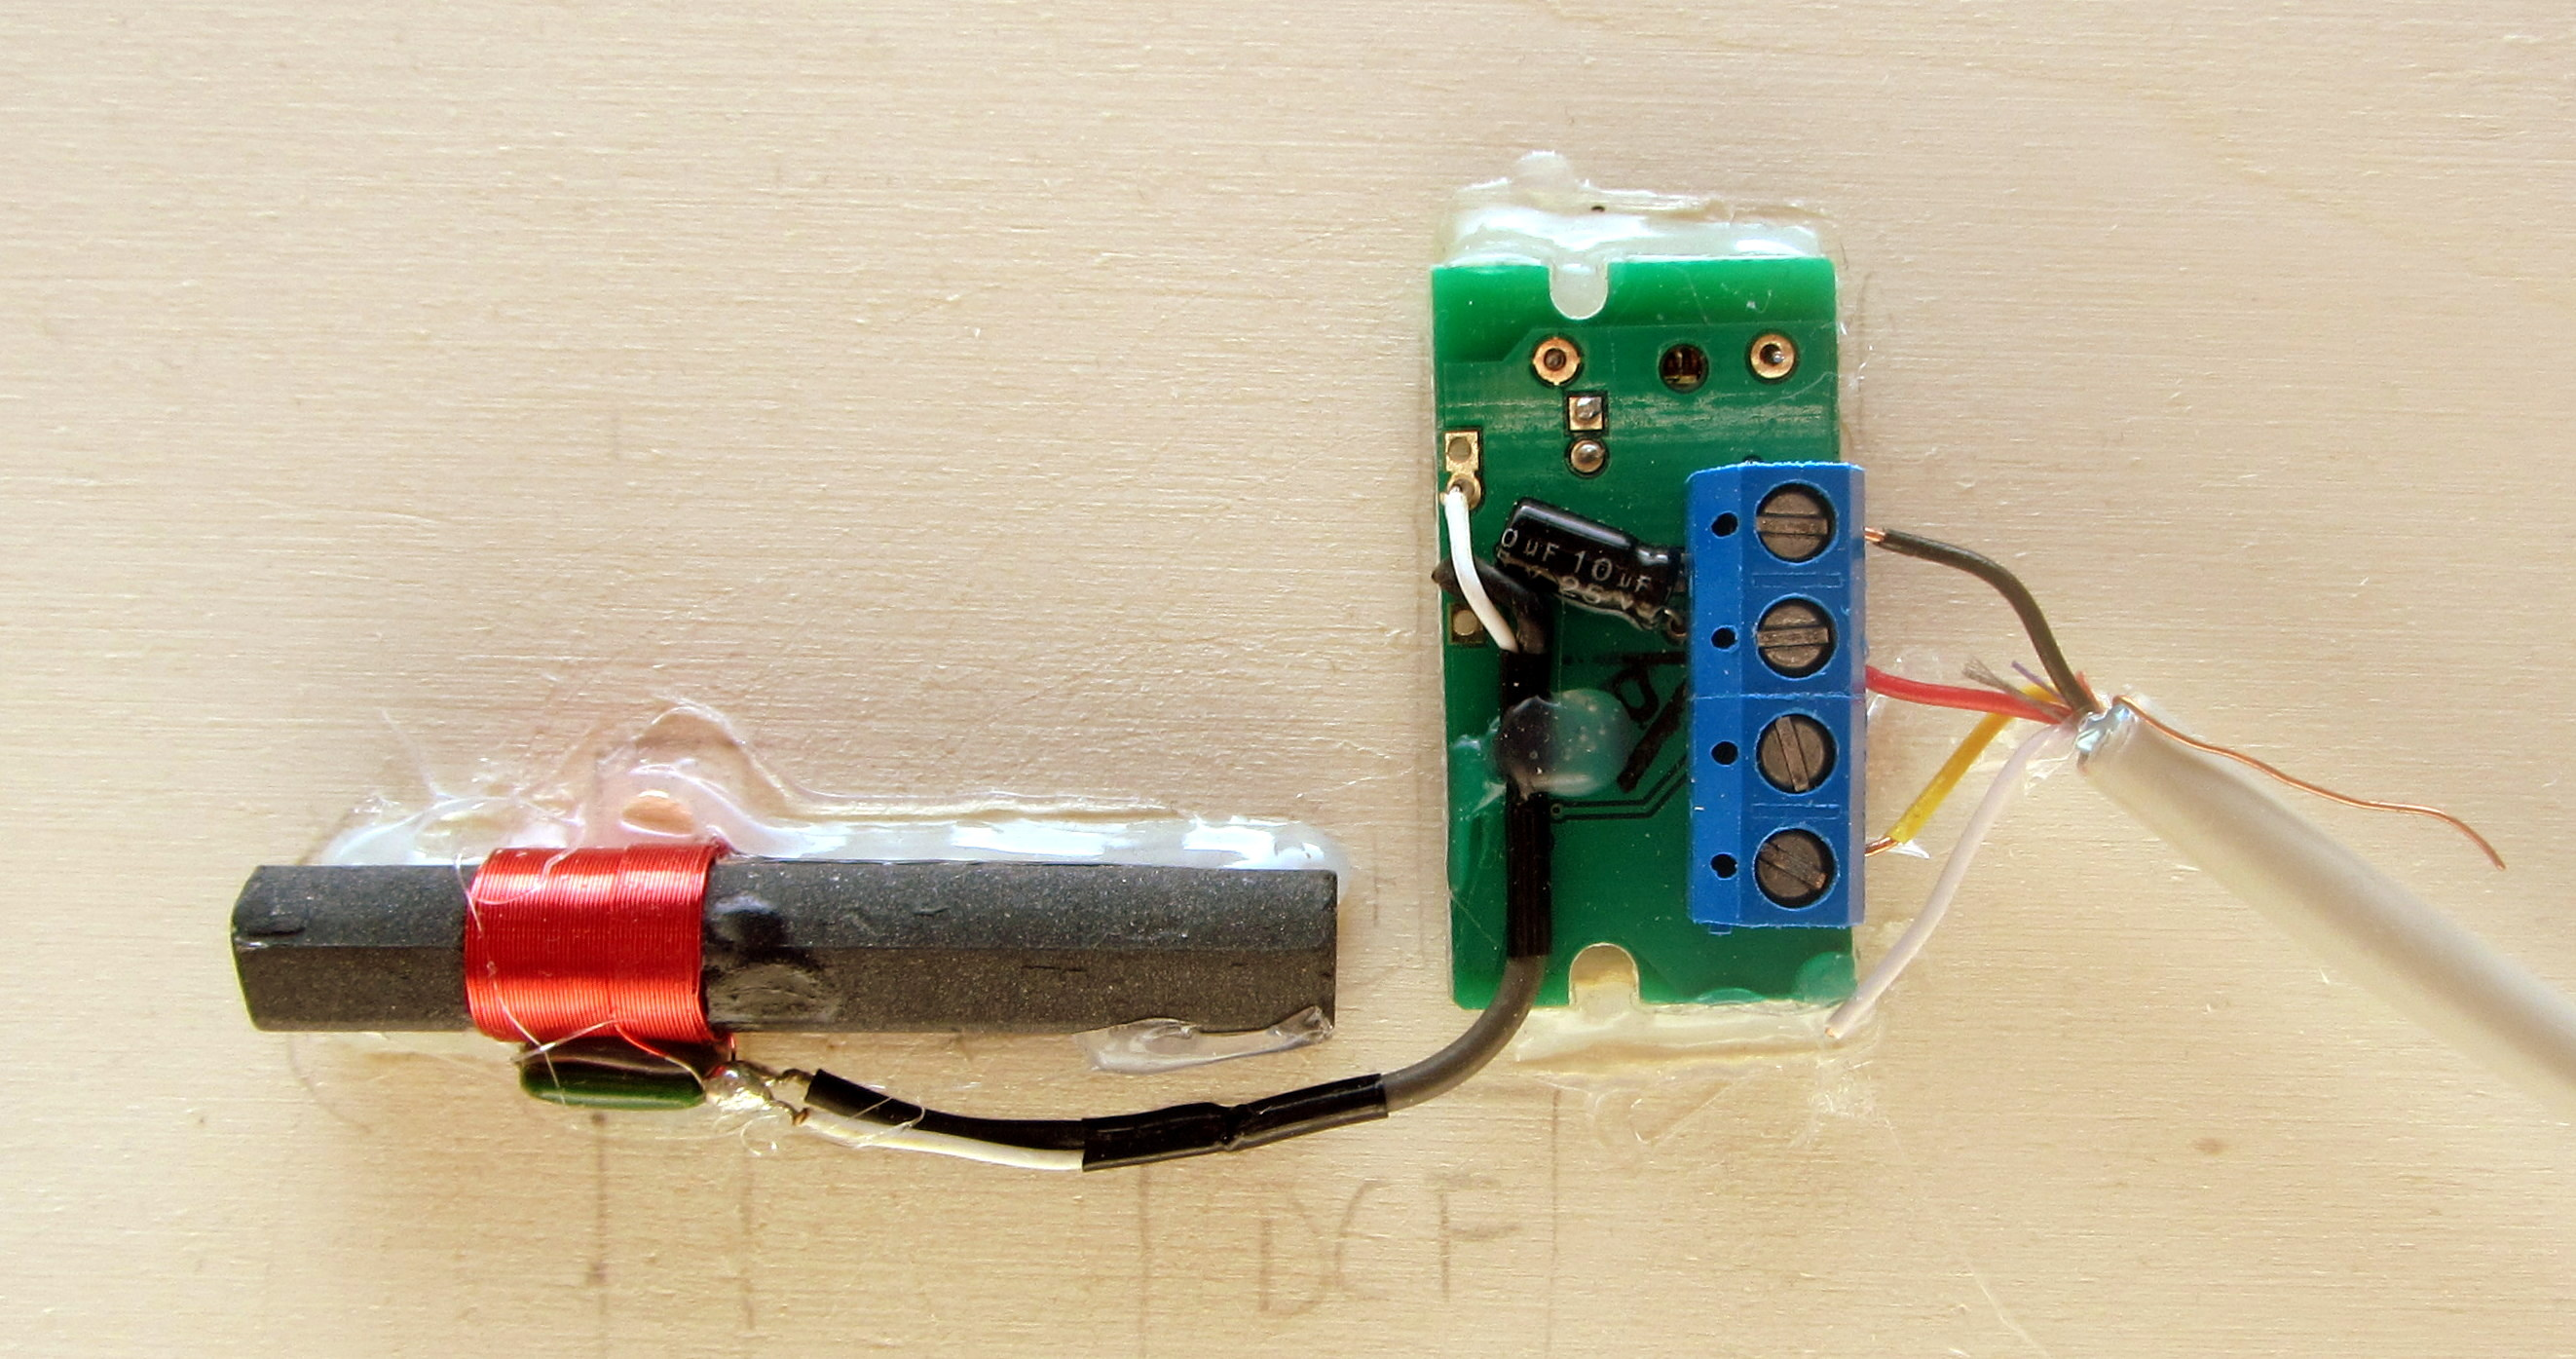
\includegraphics[width=0.75\textwidth]{images/dcf_empfaenger.jpg}}
\captionof{figure}{C-Control-DCF-Empfängerplatine von Conrad}\label{fig_dcf77}
\end{center}
%
% \begin{figure}[h]
%   \begin{center}
%   \begin{minipage}[c]{0.5\textwidth}
%         \fbox{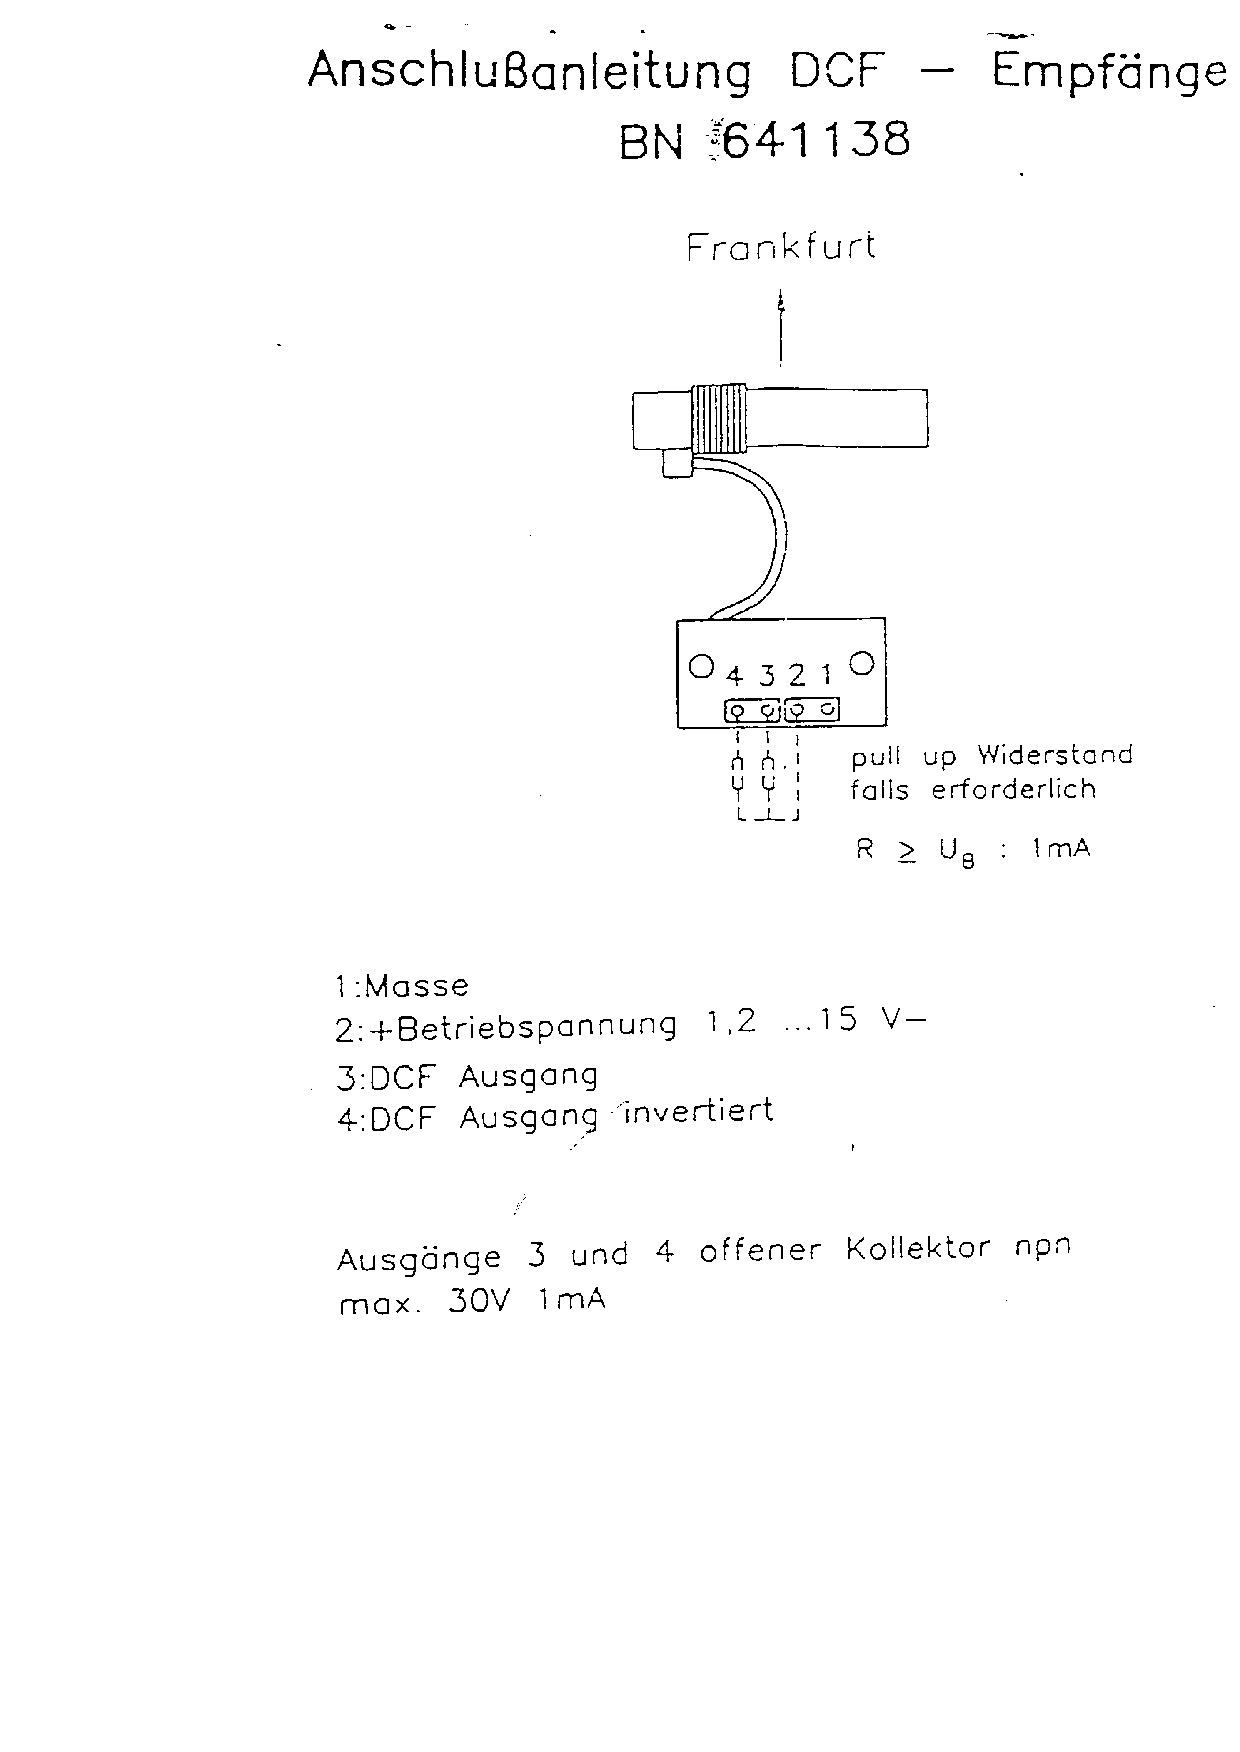
\includegraphics[width=\textwidth]{Literatur/conrad_dcf77.pdf}}
%         \caption{Anschlussanleitung DCF77 Modul\footnotemark}
%   \end{minipage}
%   \hspace{0.07\textwidth}
%   \begin{minipage}[c]{0.4\textwidth}
% Das Modul besitzt 4 Anschlüsse, welche im Anschlussplan links beschrieben sind. Es wird der \texttt{DCF Ausgang invertiert} für das Datensignal verwendet. Er ist an Microcontrollerpin PB2 angeschlossen. Damit die Uhrzeit auf jeden Fall richtig empfangen wird, ist einerseits die Ausrichtung Richtung Frankfurt wichtig sowie andererseits die Verwendung eines fehlertoleranten Codes zur Auswertung der Uhrzeit. Außerdem sollte darauf geachtet werden, das Modul nicht zu nah an Störquellen zu stellen. Als starke Störquelle stellten sich bei der Entwicklung Monitore heraus. In Abbildung TODO ist der Unterschied zwischen einem einwandfreien Signal und einem, durch einen Monitor in 2m Entfernung, gestörtem Signal abgebildet. Es ist zu erkennen, dass das Signal plötzlich im Mikrosekundenbereich gleichmäßig alterniert, also von dem ursprünglichen Signal nichts mehr zu erkennen ist.
%   \end{minipage}
%   \end{center}
% \end{figure}
%\addtocounter{footnote}{-1}%
%\footnotetext{Quelle: \url{http://www.produktinfo.conrad.com/datenblaetter/625000-649999/641138-an-01-de-Anschlussplan_DCF_Empfaengerplatine.pdf}}%
%\stepcounter{footnote}%
%

\begin{wrapfigure}{r}{0.50\textwidth}
  \vspace{-25pt}
  \begin{center}
    \fbox{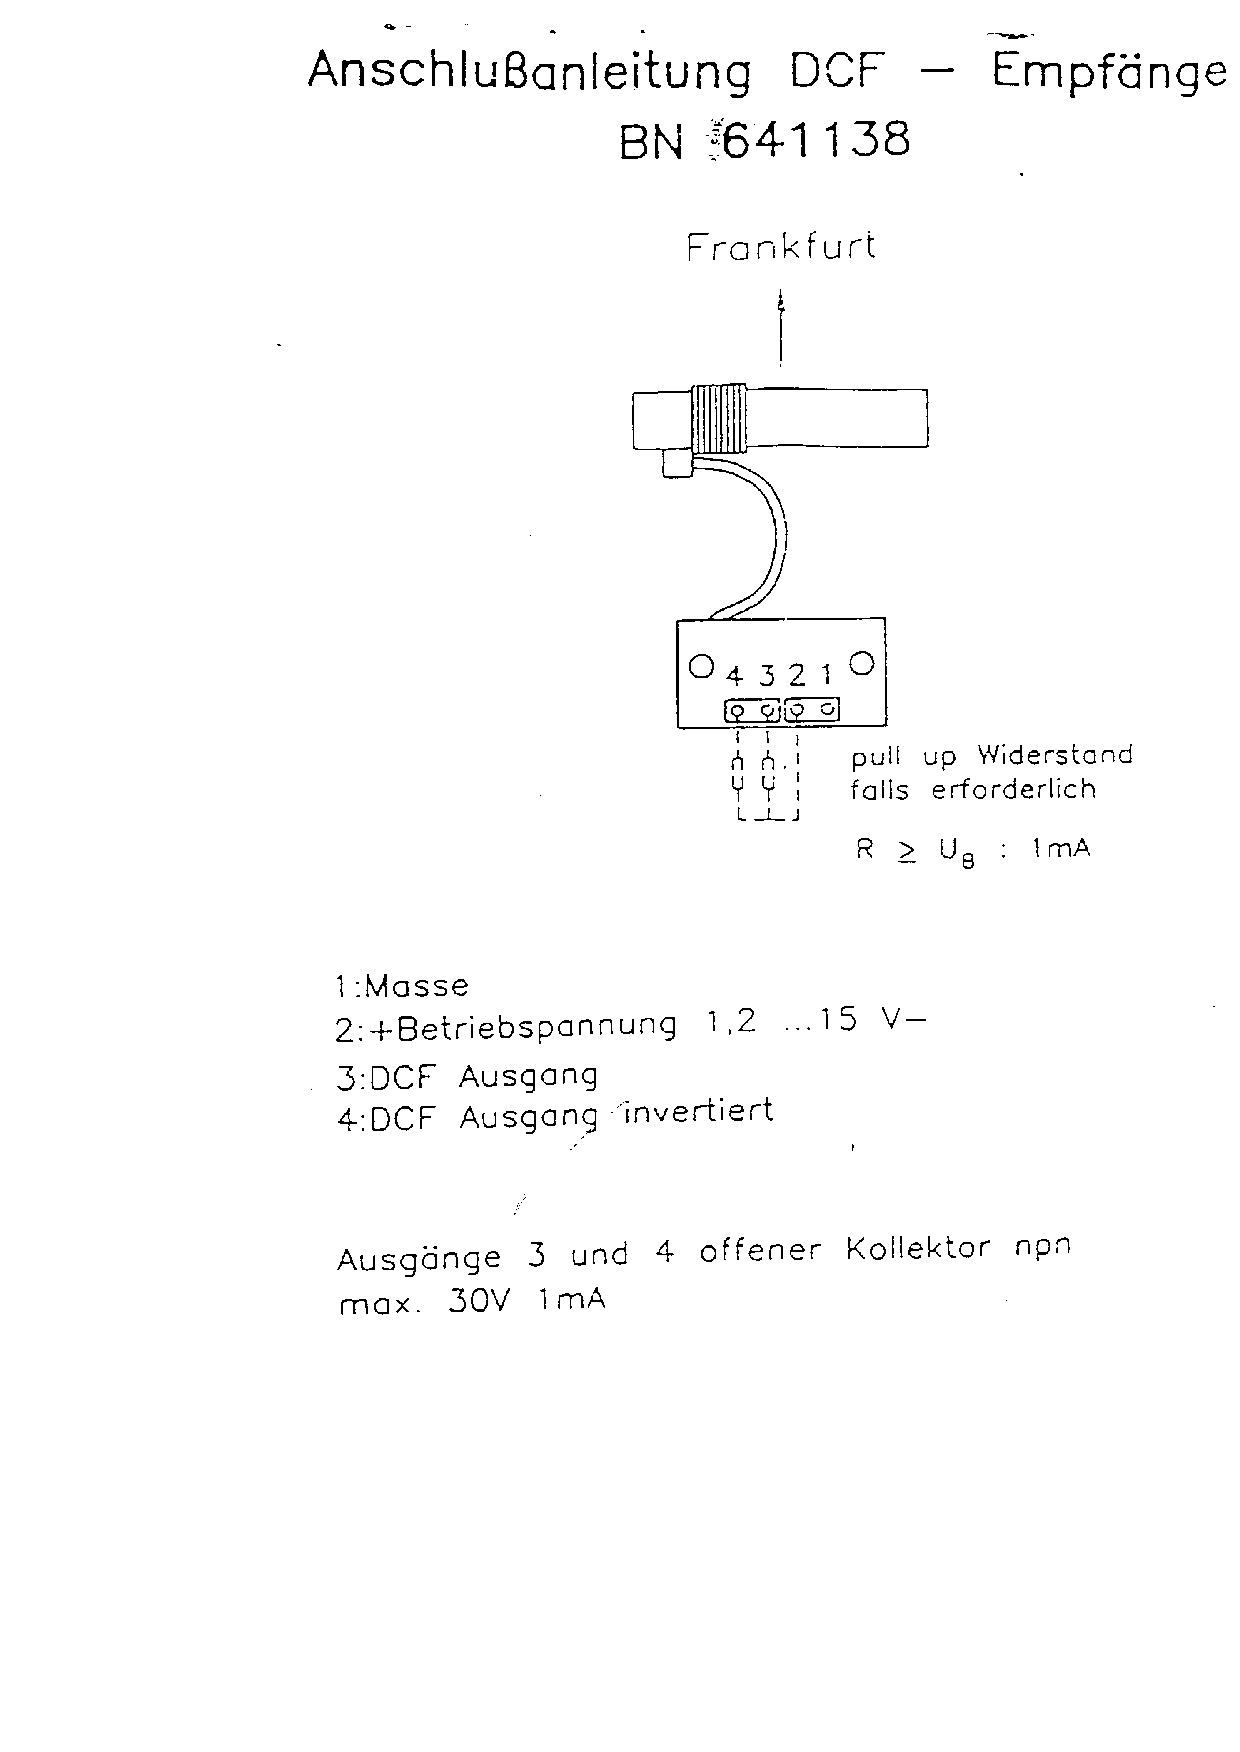
\includegraphics[width=0.45\textwidth]{Literatur/conrad_dcf77.pdf}}
  \end{center}
  \vspace{-20pt}
  \captionof{figure}{Anschlussanleitung DCF77 Modul\footnote{Quelle: \url{http://www.produktinfo.conrad.com/datenblaetter/625000-649999/641138-an-01-de-Anschlussplan_DCF_Empfaengerplatine.pdf}}}
\end{wrapfigure}
%
Das Modul besitzt 4 Anschlüsse, welche im Anschlussplan links beschrieben sind. Es wird der \texttt{DCF Ausgang invertiert} für das Datensignal verwendet. Er ist an Microcontrollerpin PB2 angeschlossen. Damit die Uhrzeit auf jeden Fall richtig empfangen wird, ist einerseits die Ausrichtung Richtung Frankfurt wichtig sowie andererseits die Verwendung eines fehlertoleranten Codes zur Auswertung der Uhrzeit. Außerdem sollte darauf geachtet werden, das Modul nicht zu nah an Störquellen zu stellen. Als starke Störquelle stellten sich bei der Entwicklung Monitore heraus. In Abbildung TODO ist der Unterschied zwischen einem einwandfreien Signal und einem, durch einen Monitor in 2 m Entfernung, gestörtem Signal abgebildet. Es ist zu erkennen, dass das Signal plötzlich im Mikrosekundenbereich gleichmäßig alterniert, also von dem ursprünglichen Signal nichts mehr zu erkennen ist.

Nachfolgend soll die Funktion \texttt{byte conrad\_state\_get\_dcf\_data()} erklärt werden. Diese Funktion ist für den Empfang der Daten des DCF77 Moduls verantwortlich. Sie als State Machine realisiert und wird beim Empfangen der Daten jede 10 ms aufgerufen. Dies wird gemacht, weil die Funktion sonst sehr lange laufen würde (der vollständige Empfang der Daten dauert im Best Case 60 Sekunden) und andere Funktionen ihre Arbeit nicht mehr verrichten können. Mit diesem Ansatz aber bleibt die Uhr reaktiv und kann beispielsweise weiterhin auf Tasterevents reagieren.
%
\begin{lstlisting}[language=C,label=dcf_state_data1,caption=Empfang des DCF77 Signals - Minutenstart erkennen]
if (i < 155) {
    /* DCF Signal unmoduliert (da es invertiert ist, ist es standartmaessig 1) */
    if (DCF_VALUE != 0) {
        i++;
        j = 0;
        DBG_LED_OFF();
    /* Wenn es moduliert ist (logisch 0) */
    } else {
        j++;

        if (j > 7) {
            i = 0;
            j = 0;
            DBG_LED_ON();
        }
    }
    return T2_WAIT;
}
\end{lstlisting}
%
In Listing \ref{dcf_state_data1} ist zunächst der erste Teil der Funktion zu sehen. Dabei geht es um das Erkennen des Minutenanfangs. Wie im DCF77 Grundlagenkapitel \ref{sec_dcfgrund} erläutert, wird das Signal beim übergang von der 59. auf die 60. Sekunde nicht moduliert, es muss also 2 Sekunden unmoduliert sein.

Die Variable i zählt die Zentisekunden, in denen das Signal unmoduliert ist. Aus Toleranzgründen wird lediglich geschaut, ob i den Wert von 155 übersteigt, statt 200 (= 2 s). Es kann nämlich passieren, dass das Signal zufällig genau zum Messzeitpunkt leicht abfällt. Deshalb werden auch Werte von j, welches die modulierten Zentisekunden misst, von weniger als 70 ms ignoriert. Somit werden Ungenauigkeiten durch, die durch Tests ermittelten, Werte von 155 und 7 ziemlich zuverlässig vermieden.

Wie zu erkennen ist, gibt es keine Schleife, sondern lediglich sequentiellen Code, der auf jeden Fall returned (siehe Zeile 17). Es gibt die folgenden Return-Codes:
%\begin{description}
%\item[T2\_WAIT] Resettet den Counter von Timer2, sodass genau 10 ms gewartet wird
%\item[ERROR] Bricht den Messvorgang ab, weil ein Fehler aufgetreten ist
%\item[SUCCESS] Alle 60 Bits wurden gemessen. Dabei wurde kein Fehler erkannt
%\end{description}
%
\begin{list}{\ding{42}}
{\setlength{\topsep}{0cm}
\setlength{\itemsep}{0.2cm}
\setlength{\leftmargin}{3cm}
\setlength{\labelwidth}{3cm}
\setlength{\labelsep}{0cm}
\renewcommand{\makelabel}[1]{\textbf{\textsf{\normalsize #1} }}}
\item[T2\_WAIT] Resettet den Counter von Timer2, sodass genau 10 ms gewartet wird
\item[ERROR] Bricht den Messvorgang ab, weil ein Fehler aufgetreten ist
\item[SUCCESS] Alle 60 Bits wurden gemessen. Dabei wurde kein Fehler erkannt
\end{list}
%
%\lstinputlisting[label=samplecode,caption=A sample]{sourceCode/HelloWorld.java}
%
%
In diesem Fall wird der Returncode \texttt{T2\_WAIT} verwendet, damit die Funktion nach 10 ms nochmals aufgerufen wird und die Messung fortgesetzt werden kann.
%
\begin{lstlisting}[language=C,label=dcf_state_data2,caption=Empfang des DCF77 Signals - Sekunde analysieren]
if (is_start_of_sec) {
    /* Pausiere bis zum modulierten Signal */
    if (DCF_VALUE != 0) {
        return T2_WAIT;
    }
    is_start_of_sec = false;
}
if (k < 95) {
    if (DCF_VALUE != 0) {
        unmodulated++;
    } else {
        if (k < 40) {
            modulated++;
        }
    }
    k++;
    return T2_WAIT;
}
\end{lstlisting}
%
Der nächste Schritt (siehe Listing \ref{dcf_state_data2}) ist das Analysieren jeder Sekunde, also das Zählen der modulierten und nicht-modulierten Signale. Dazu wird zunächst gewartet, bis die Sekunde anfängt, also das erste modulierte Signal auftritt (Zeile 3), anschließend wird 95 \% der Sekunde analysiert. Die letzten 5 \% sind Toleranz, damit die nächste Sekunde sicher erkannt werden kann. Modulierte Signale treten nur in den ersten 200 ms einer Sekunde auf, deshalb werden sie nur am Anfang gezählt, aber aus Toleranzgründen innerhalb der ersten 400 ms (Zeile 12). Auch hier wird nach jeder Messung die Routine mit \texttt{T2\_WAIT} verlassen (Zeile 17).
%
\begin{lstlisting}[language=C,label=dcf_state_data3,caption=Empfang des DCF77 Signals - Sekunde analysieren]
if (unmodulated > 50 && unmodulated < 140) {
    /* Wenn moduliert zwischen 50 und 140 ms, liegt logisch 0 an */
    if (modulated > 5 && modulated < 14) {
        dcf_data[secs] = 0;
    /* Zwischen 150 ms und 240 ms, liegt logisch 1 an */
    } else if (modulated > 15 && modulated < 24) {
        dcf_data[secs] = 1;
    /* sonst ist es ungueltig */
    } else {
        return ERROR;
    }
} else {
    return ERROR;
}
/* Bereite die naechste Sekunde vor */
secs++;
is_start_of_sec = true;
k = 0;
modulated = 0;
unmodulated = 0;

return SUCCESS;
\end{lstlisting}
%
Als letztes werden die Daten ausgewertet, also geprüft ob logisch eine 0 oder 1 gemessen wurde. Dazu wurden Zahlen gewählt, die sich durch Tests bewährt haben (siehe Listing \ref{dcf_state_data3}). Bei fehlerhaften Daten wird \texttt{ERROR} zurückgegeben (Zeile 10 und 13) und die gesamte Messung abgebrochen. Sind die Daten gültig, wird die State Machine auf den Anfangszustand jeder Sekunde gesetzt (Zeilen 16 -- 20) und \texttt{SUCCESS} zurückgegeben und damit die Auswertung der nächsten Sekunde begonnen.

Wie zu sehen ist, werden statt diskreten Werten immer Bereiche angenommen, in denen ein bestimmter Wert liegen muss. Dies ist durch die funkbedingten Ungenauigkeiten unbedingt notwendig. Es erforderte einige Tests, bis die passenden Werte gefunden wurden, um einen passablen Empfang zu erreichen, was letzten Endens jedoch gelang und zu einem korrekt funktionierendem Funkmodul für die Digitaluhr führte.
%
\subsection{LED Matrix}
\subsubsection{Schaltung und Hardware}
\begin{center}
	\includegraphics[width=\textwidth]{images/LED_Matrix.png}
	\captionof{figure}{LED Matrix Draufsicht}
\label{led_oben}
\end{center}
Die LED Matrix dient der Uhr als Display. Es werden $7*17=119$ blaue
LEDs\footnote{LED Spexx TODO} verwendet. Die LEDs haben einen Abstand von $45 mm$ und werden durch ein Gitter aus Sperrholz voneinander getrennt, so dass
Pixel entstehen. Durch das Multiplexen der Zeilen kann jede LED unabhängig
gesteuert werden.

Die Anoden der Reihen sind jeweils verbunden und an die Schieberegister TODO REF
angeschlossen. Die Kathoden sind Zeilen verbunden und über die Mosfets vom
Mikrocontroller geschaltet. Eine Ausnahme bildet Reihe 17, da die 2
Schieberegister nur 16 Ausgänge bieten wurde diese direkt an den Mikrocontroller
angeschlossen.
\begin{center}
	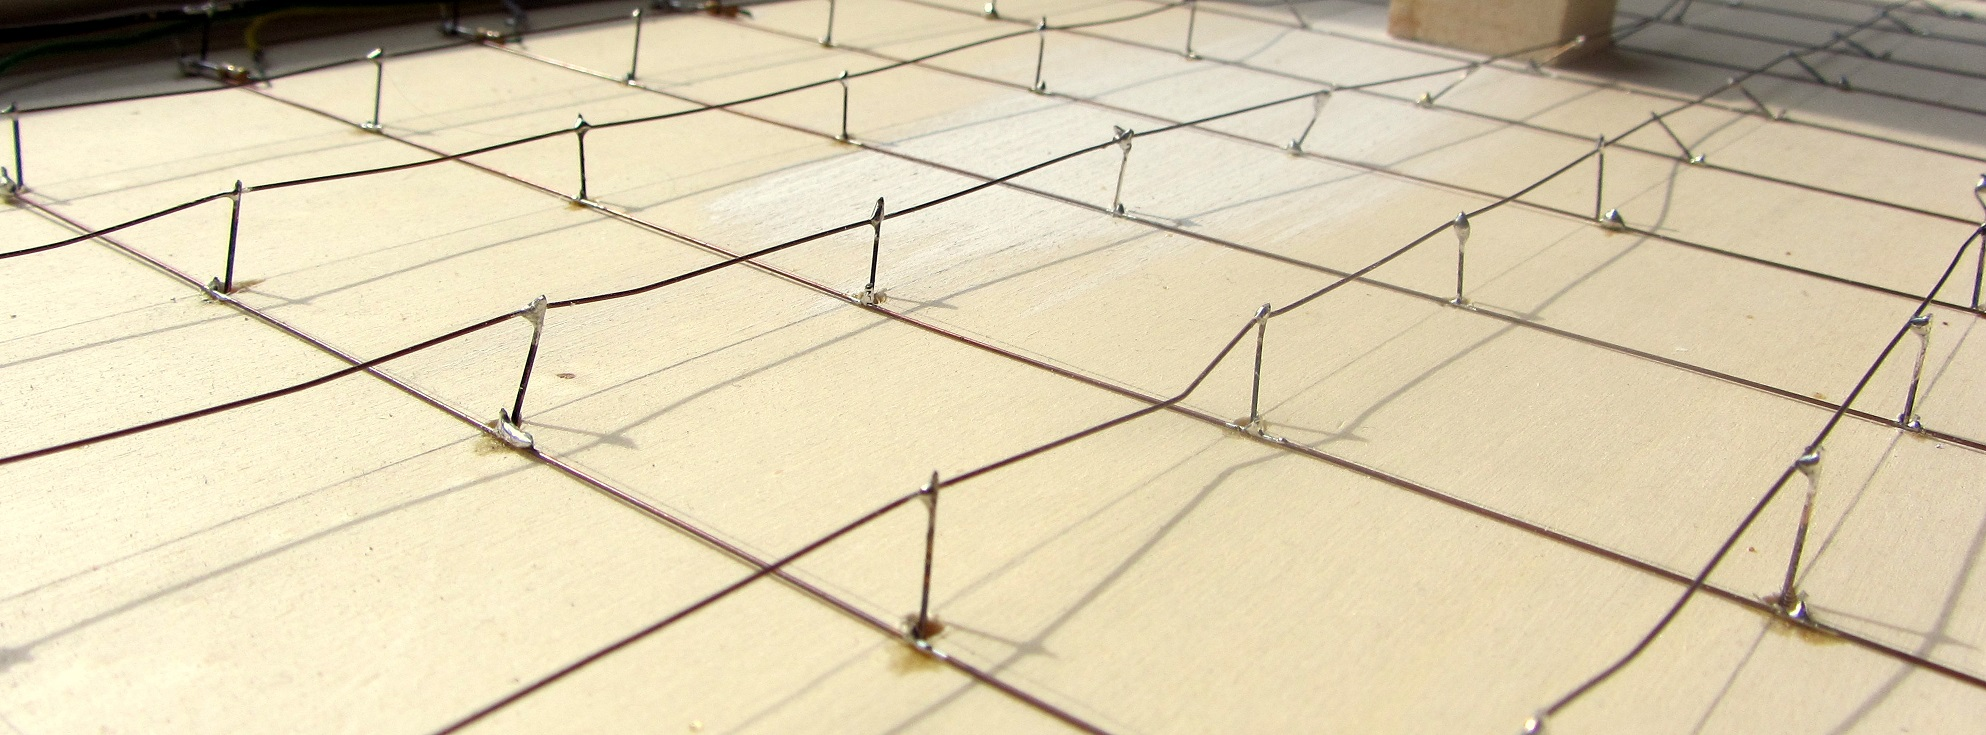
\includegraphics[width=\textwidth]{images/unterseite_drahtgitter.jpg} 
\captionof{figure}{LED Matrix Verdrahtung, Anoden aufliegend und Kathoden
schwebend verbunden}
\end{center}
\label{led_matrix_verdrahtung}

\begin{center}
	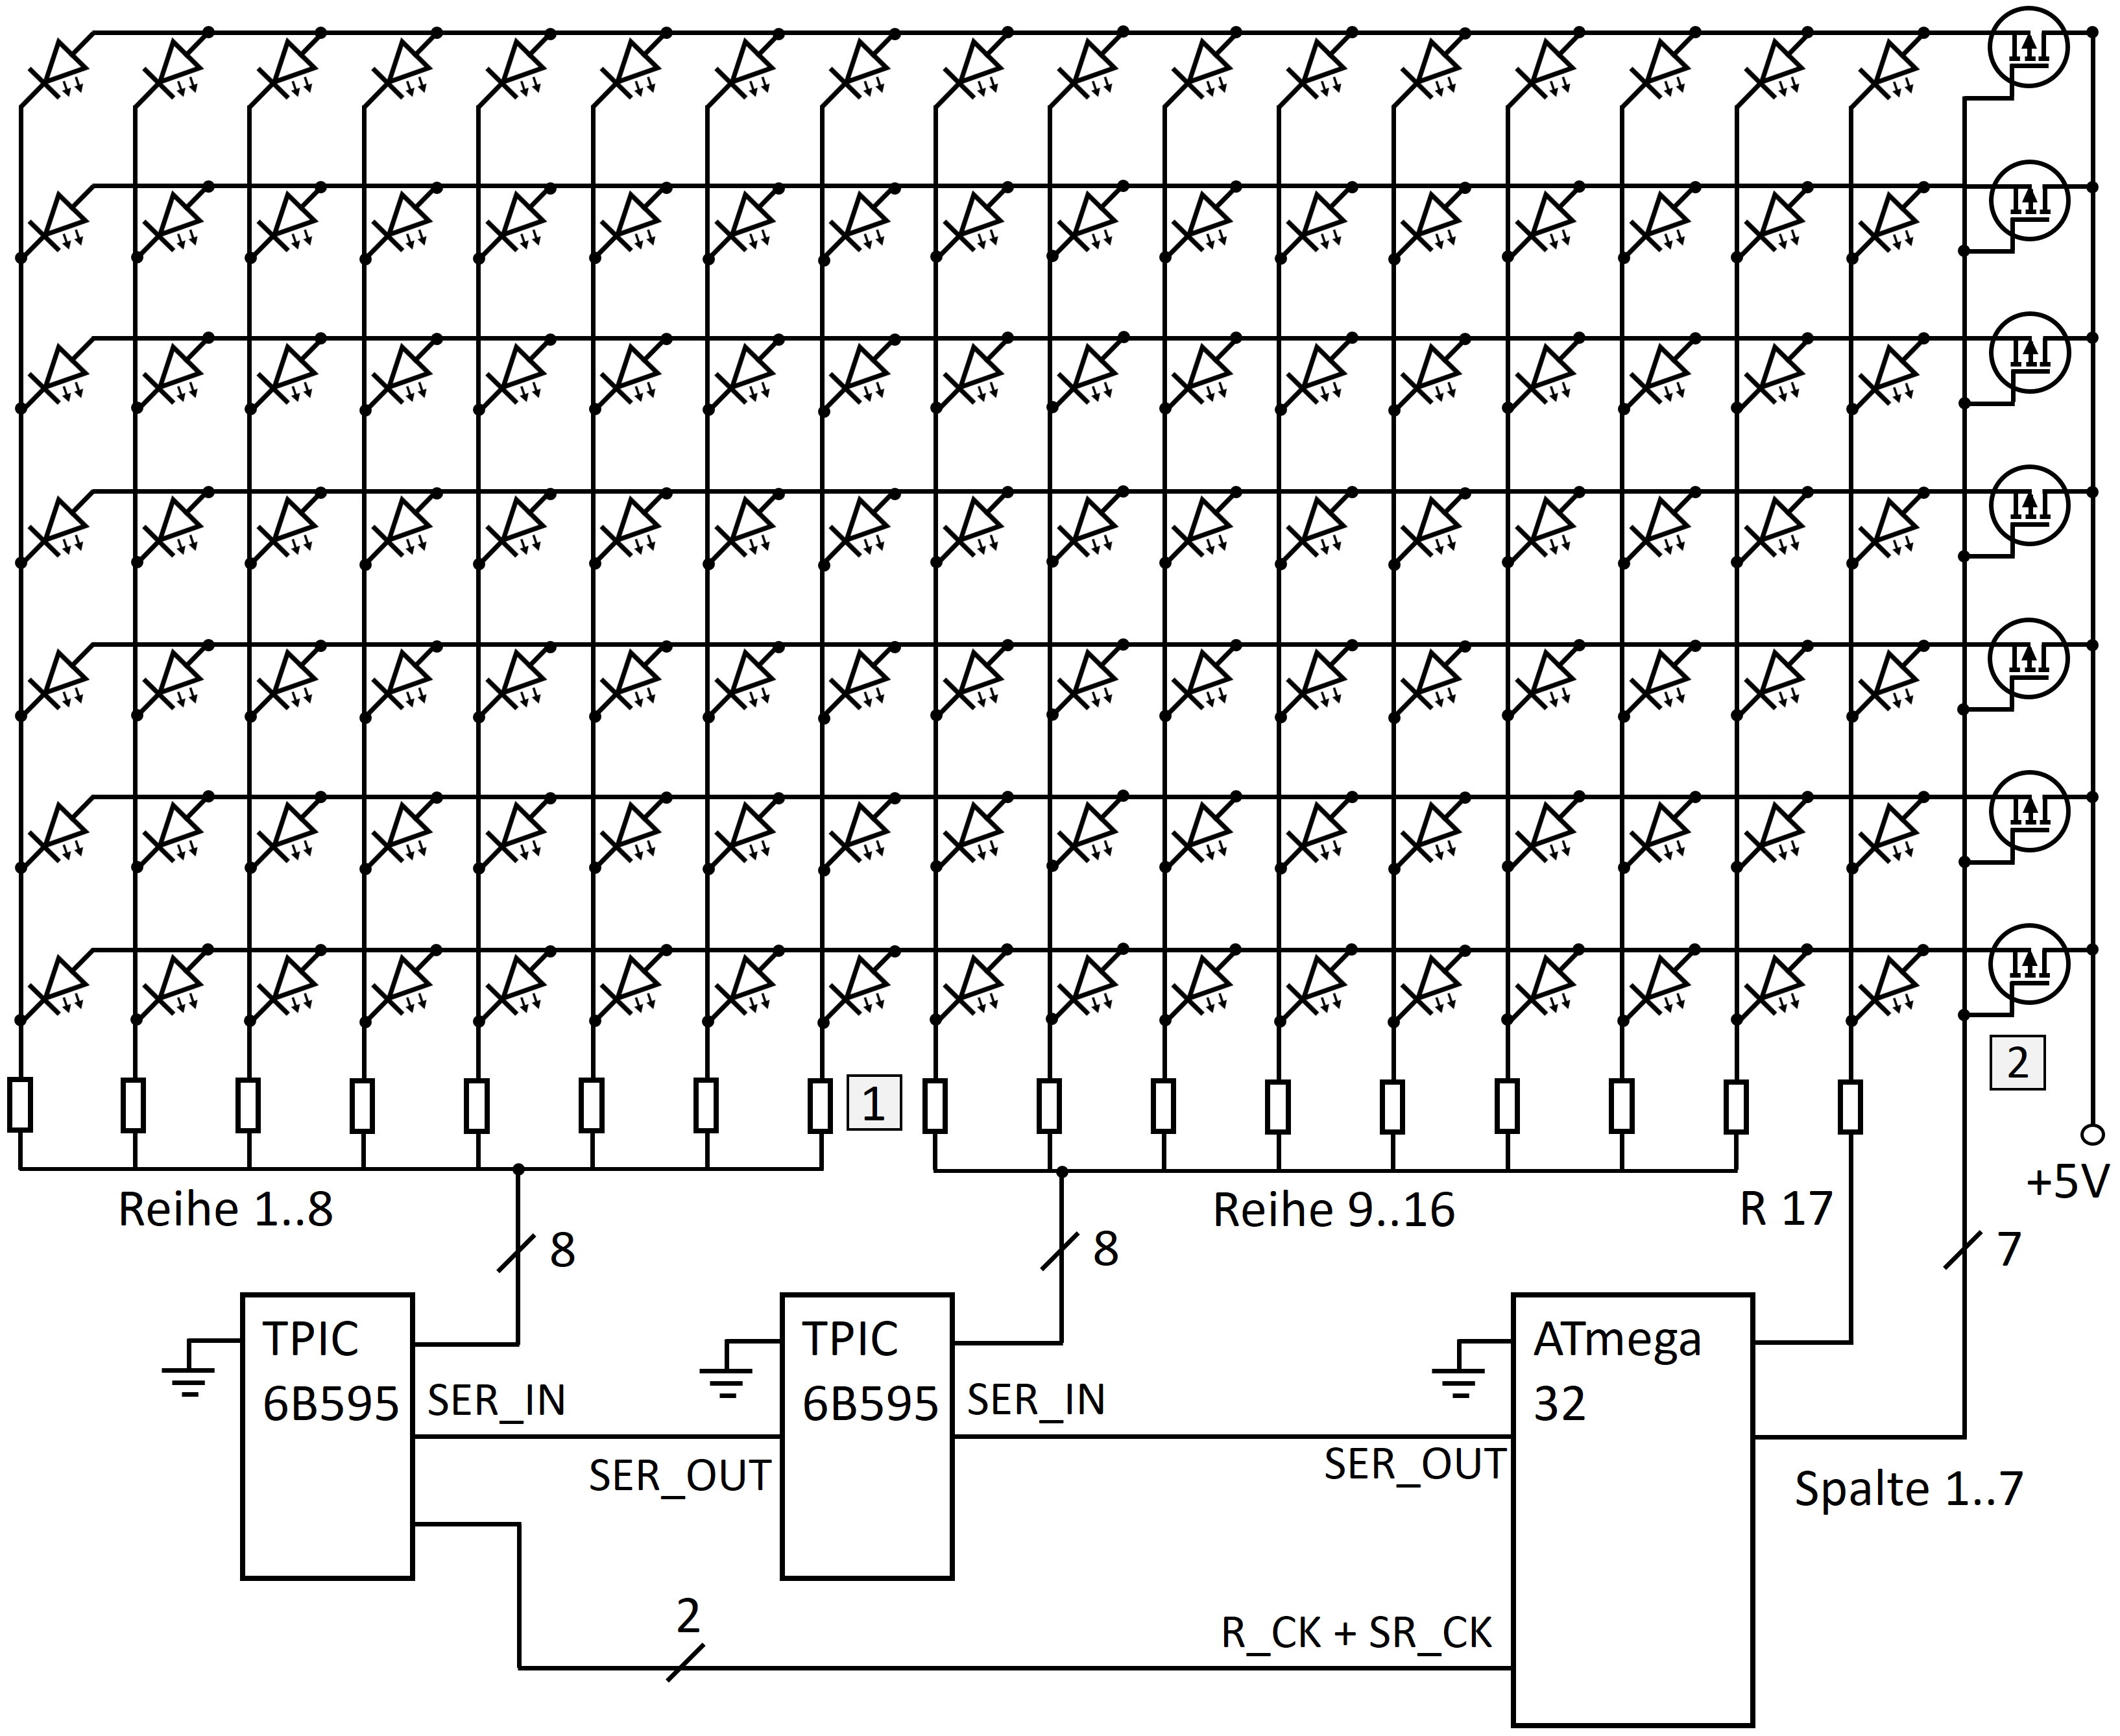
\includegraphics[width=\textwidth]{skizzen/led_matrix_schaltplan.png} 
\captionof{figure}{LED Matrix Schaltplan, 1: LED
Vorwiderstände, 2: P-Kanal Mosfets \mbox{IRLZ24N}}
\end{center}
\label{led_matrix_schaltplan}

Durch die Ansteuerung als Matrix werden nur 24 Leitung von der LED Anzeige zur
Hauptplatine benötigt. Da der Mikrocontroller auf seinen Logikausgängen nicht
die benötigte Leistung bereitstellen kann wird die Spannung durch die P-Kanal
Mosfets vom Typen IRLZ24N geschalten.

Um weitere Pins am ATmega einzusparen werden die Reihen (abgesehen von Reihe 17)
mittels Schieberegister gesteuert. Die beiden Schieberegister vom Typen
TPIC6B595 können dauerhaft Ströme bis zu 150mA pro Pin und 500mA Gesamtstrom gegen GND
schalten.\footnote{vgl. \cite{6b595}, S. 1} Die Kommunikation zwischen ATmega
und den Schieberegistern erfolgt über das SPI Interface, welches sehr einfach mit Daten gefüllt werden kann und
diese unabhänig vom eigentlichen Programmablauf an die Schieberegister schickt.

\begin{wrapfigure}{r}{0.5\textwidth}
  \vspace{-25pt}
  \begin{center}
    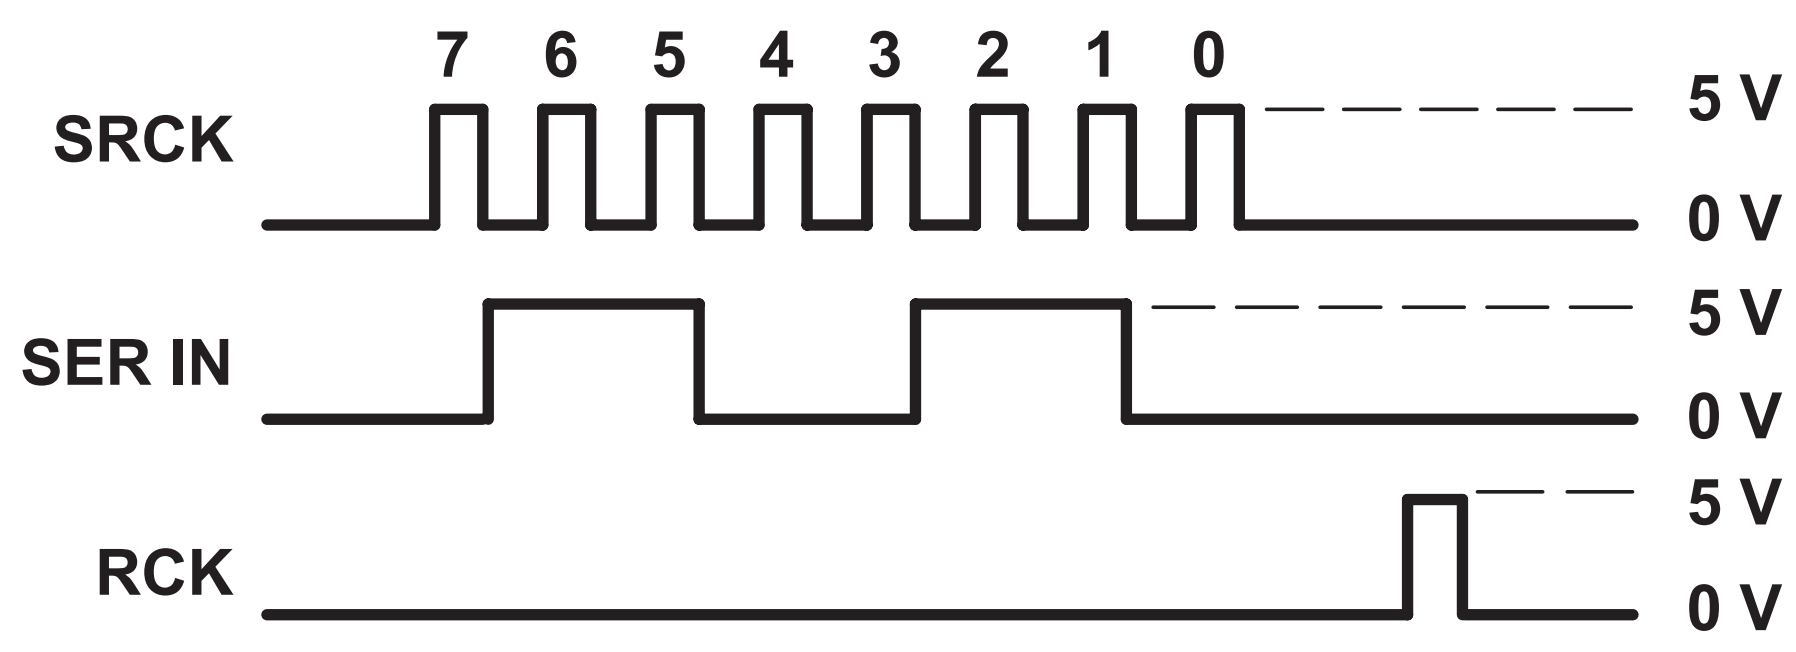
\includegraphics[width=0.48\textwidth]{skizzen/schieberegister_linien.png}
  \end{center}
  \vspace{-20pt}
  \captionof{figure}{Füllen des Schieberegisters\footnote{\cite{6b595}, S. 5}}
\end{wrapfigure}

Das SPI Interface wird über 3 Leitungen realisiert: SER IN als Datenleitung,
SRCK zur Taktübertragung, RCK um die Daten vom Schieberegister auf die
Ausgänge zu legen. Das zweite Schieberegister wird parallel an RCK und SRCK
verbunden, und der serielle Ausgang des ersten Schieberegisters SER OUT wird mit
SER IN des zweiten Schieberegister verbunden, durch diese Schaltung erreicht man
quasi ein 16-bittiges Schieberegister.
Insgesamt benötigt das Display somit 11 Pins am Mikrocontroller: 3 für die
Schieberegisteransteuerung, 7 für die Ansteuerung der Mosfets sowie eine Leitung
um Reihe 17 zu schalten.
\subsubsection{Software}
Im folgenden wird die Ansteuerung der LED Matrix beleuchtet, diese findet in der
Methode \texttt{drawWithBrightness(void)}. Diese gibt jeweils 1 komplette Zeile aus und wird periodisch aufgerufen. Zu Anfang wird der aktuelle \texttt{cmp}
Vergleichswert mit der global eingestellten Helligkeit \texttt{brightness}
verglichen. Wenn \texttt{brightness} größer als dieser Wert ist bleiben die LEDs
im Aufruf dunkel, was für die dynamische Helligkeitsanpassung von Nöten ist. 

Wenn gezeichnet werden soll wird auf die Bilddaten im Array \texttt{data}
zugeriffen und für jedes Pixel überprüft ob dieses aktiv sein soll, die Pixel
werden durch Schiebeoperttionen nacheinander in die \texttt{output} Varible
geschrieben. 

\begin{lstlisting}[language=C,label=dcf_state_data2,caption=Zeichenmethode zur
Ansteuerung der LED Matrix: Teil 1] 
/*Draws all the pixel with the brigtness of
the global brightness variable*/ static inline void drawWithBrightness(void){ 
byte output=0;
	if(brightness>cmp){
		byte i=0;
		/* The first output Byte */
		for(i=0;i<8;i++){
			output = output<<1;
			if(data[row][i]>0){
				output++;
			}
		}
\end{lstlisting} 

Der Inhalt der \texttt{output} Variable wird anschliesend in das
\texttt{SPDR} Register geschrieben, welches den Buffer der SPI Schnittstelle
darstellt. Im Hintergrund beginnt nun das SPI Modul des ATmega die Daten an das
Schieberegister zu übertragen. Während dessen werden die Pixeldaten für Reihe
9--16 verarbeitet. Anschließend wird gewartet bis die Übertragung zum
schieberegister abgeschlossen ist und der neue \texttt{output} Wert in das
\texttt{SPDR} register geschrieben.

\begin{lstlisting}[language=C,label=dcf_state_data2,caption=Zeichenmethode zur
Ansteuerung der LED Matrix: Teil 2]
		/* output to SPI-Register */
		SPDR = output;
		output = 0;
		/* Second output Byte */
		for(;i<16;i++){
			output = output<<1;
			if(data[row][i]>0){
				output++;
			}
		}
		/* Wait for SPI transmission complete*/
		while(!(SPSR & (1<<SPIF)));
		/* output to SPI-Register */
		SPDR = output;
\end{lstlisting} 

Die Ausgabe von Reihe 17 unterscheidet sich deutlich da der Mikrocontrollerpin
auf dem selben Port wie die Mosfets liegt. Auserdem muss hier GND anliegen wenn
die LED aktiviert sein soll. Deshalb wird \texttt{output} mit \texttt{128}
(achtes Bit im Byte) initialisiert und wenn das Pixel aktiv ist mit \texttt{0}
überschrieben.

Im \texttt{else}-Fall wenn alle LEDs aus bleiben sollen werden Nullen in die
Schieberegister geschoben und das achte Bit von \texttt{output} mit 1
beschrieben.
\begin{lstlisting}[language=C,label=dcf_state_data2,caption=Zeichenmethode zur Ansteuerung der LED Matrix: Teil 3] output = 128;

		/* Last Bit direct on microcontroller pin */
		if(data[row][i]>0){
			output=0;
		}
		while(!(SPSR & (1<<SPIF)));
	}else{
		/* output to SPI-Register */
		SPDR = 0;
		/* Wait for SPI transmission complete*/
		while(!(SPSR & (1<<SPIF)));
		SPDR = 0;
		while(!(SPSR & (1<<SPIF)));

		output=128; //LED 16 aus!
	}
\end{lstlisting} 
Zu letzt muss die RCK Leitung der Schieberegister auf Low und anschliessend auf
High geschalten werden sowie der Mosfet der aktuellen Zeile aktiviert werden.
Die Mosfets schalten durch wenn sie mit Low beschalten werden. Um während des
Schaltens im Schieberegister Falkern auf der Anzeige zu verhindern werden zuerst
alle Mosfets ausgeschalten, dann die Schieberegisterinhalte auf die
Schieberegisterausgänge übernommen und anschliessend der Mosfet der Zeile
aktiviert. 

Abschliessend wird die Zeilenummer für den nächsten Aufruf der Methode nach oben
gesetzt und wenn ein komplettes Bild gezeichnet wurde \texttt{row==7} wird der
\texttt{cmp} Wert um 16 erhöht, dadurch existieren 16 verschiedene
Helligkeitstufen.

\begin{lstlisting}[language=C,label=dcf_state_data2,caption=Zeichenmethode zur Ansteuerung der LED Matrix: Teil 4]

	/* RCK auf null ziehen */
	PORTB &= 0b11101111;
	/* Alle Mosfets aus, PD7 unbelegt */
	PORTD = 0xFF;//
	/* RCK auf high */
	PORTB |= 0b00010000;
	/* Mosfet wieder an */
	PORTD = states[row++] + output;
	if(row == 7){
		row = 0;
		/* Increment cmp-variable */
		cmp+=16;
	}
}
\end{lstlisting}

\subsection{Helligkeitssensor}
Ein Fotoresitor (Lichtabhängier Widerstand, kurz LDR für Light Dependend Resistor) bildet einen Teil eines Spannugteilers. Die innerhalb des Spanungsteilers anliegende Spannung wird dann vom Mikrocontroller mit Hilfe des AD-Wandlers ausgewertet.
Der verwendete Fotoresisor besitzt nominal einen Dunkelwiderstand von $100 k\Omega$ .
Um den Widerstandsverlauf besser abschätzen zu können wurden Messungen vorgenommen.
\begin{figure}[h]
  \begin{center}
  \begin{minipage}[b]{0.3\textwidth}
        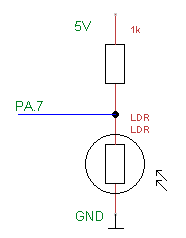
\includegraphics[height=4.5cm]{skizzen/helligkeitssensor_schmatic.png}
        \caption{Spannungsteiler des LDRs}
  \end{minipage}
  \hspace{0.07\textwidth} 
  \begin{minipage}[b]{0.6\textwidth}
    \begin{tabular}[h]{||l | l||}
	  \hline \hline
	  Dunkelheit& $70 k\Omega$ \\ \hline
	  Zimmerhelligkeit & $3 k\Omega$ \\ \hline
	  Schreibtischlampe 50cm Abstand& $500 \Omega$ \\ \hline
	  Schreibtischlampe 10cm Abstand& $90 \Omega$ \\ \hline
	  Schreibtischlampe 2cm Abstand& $30 \Omega$  \\
	  \hline\hline
    \end{tabular} 
    \label{Modellversuch} 
    \captionof{table}{Widerstandmessung des LDR}
  \end{minipage}
  \end{center}
\end{figure}
%
\subsection{Temperatursensor}
Als Temperatursensor wurde der DS18S20\footnote{\url{http://www.maximintegrated.com/datasheet/index.mvp/id/2815}} von Maxim Integrated verwendet. Dieser verwendet das 1-Wire\textsuperscript{\textregistered}-Protokoll\footnote{\url{http://www.maximintegrated.com/products/1-wire/flash/overview/index.cfm}}, sodass nur ein Datenpin vonnöten ist, worüber Befehle gesendet sowie Daten empfangen werden.

Der 1-Wire-Bus ermöglicht die Verwendung mehrerer Geräte an der Datenleitung, wobei jedes Gerät über seine eindeutige 64-Bit ID angesprochen wird. Da bei diesem Projekt lediglich ein DS18S20 verwendet wird, kann die Ansteuerung der eindeutigen ID weggelassen werden und alle Geräte auf dem Bus angesprochen werden, da keine Kollision entstehen kann.

Der Temperatursensor wird wie in Grafik \ref{fig_tempsensor} angeschlossen. Die Datenleitung wird über einen $4,7 k\Omega$ Pullup-Widerstand mit der Spannungsquelle verbunden, sowie an Pin PA6 des Microcontrollers angeschlossen.
%
\begin{figure}[htp]
\centering
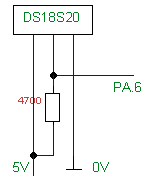
\includegraphics{skizzen/temperatursensor_schematic.png}
\caption{Schaltung für den 1-Wire Temperatursensor}\label{fig_tempsensor}
\end{figure}
%
Für das 1-Wire-Protokoll ist ein genaues Timing unabdingbar, deshalb müssen bei jeglicher Kommunikation mit dem DS18S20 alle Interrupts ausgeschaltet werden. Da die längste Kommunikation am Stück der Reset-Pulse mit $960 \mu s$ ist, ist das Auschalten der Interrupts für die Funktionalität der Uhr nicht beeinträchtigend.

Das Protokoll sieht vor, dass jede Kommunikation mit einem Reset-Pulse startet. In Abbildung \ref{fig_resettiming} 
ist das genaue Timing des Reset-Pulses zu erkennen. Zunächst muss der Master, also hier der Microcontroller den Bus für mindestens $480 \mu s$ auf Low ziehen. Nach Freigabe des Busses sorgt der Pullup-Widerstand dafür, dass der Bus wieder auf High gesetzt wird. Anschließend zieht der Sensor den Bus nach $15 \mu s$ bis $60 \mu s$ nach der ansteigenden Flanke für $60 \mu s$ bis $240 \mu s$ auf Low. Dies signalisiert dem Master, dass ein Gerät am Bus hängt und einsatzbereit ist.\footnote{\cite{ds18s20}, Seite 13}

In der weiteren Kommunikation wird nun das \texttt{SKIP ROM} Kommando benutzt, welches bedeutet, dass die 64-Bit ID weggelassen werden kann und alle Geräte (hier nur eins) angesprochen werden. Nun kann der DS18S20 mit dem \texttt{CONVERT TEMP} Kommando dazu aufgefordert werden, die Temperatur zu messen und digital zu konvertieren. Dies macht er nicht permament um Strom zu sparen. Nach einer Konvertierungszeit von mindestens $700 ms$ kann die Temperatur ausgelesen werden. Dazu muss erneut ein Reset- sowie ein Skiprom-Kommando gesendet werden, um dann mit \texttt{READ SCRATCHPAD} die eigentliche Temperatur zu erhalten.\footnote{Genaue Beschreibung der Kommandos siehe \cite{ds18s20} Seite 10ff}
%
\begin{figure}[htp]
\centering
\centerline{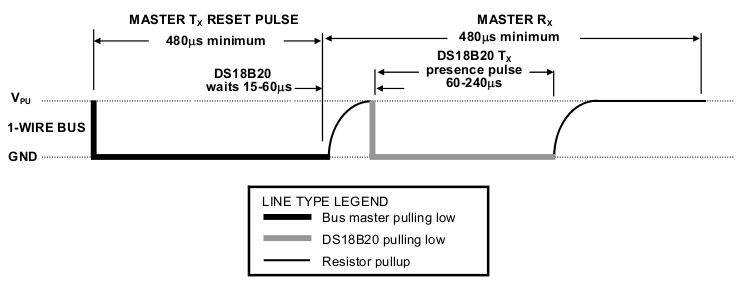
\includegraphics[width=\linewidth]{skizzen/temperatur_reset.png}}
\caption{Reset-Pulse Timing Diagramm\footnote{\cite{ds18s20}, Seite 13}}\label{fig_resettiming}
\end{figure}
%
\subsection{Gehäuse}
%TODO
%
Ziel war es ein optisch ansprechendes, sowie funktionales Gehäuse zu kreieren. 

Als problematisch stellte sich die Zielsetzung der flachen Bauart heraus. Denn um eine gleichmässige Lichtverteilung innerhalb eines Pixels zu erreichen, muss ein relativ großer Abstand zur LED gegeben sein. Durch praktisches Testen ergab sich für die verwendeten LEDs ein idealer Abstand von .%TODO eventuell wirklich probieren 
Außerdem muss verhindert werden, dass die offenliegende Verdrahtung der LED-Matrix zu Kurzschlüssen führt. Im Besonderen ist hier das Netzteil zu nennen, da hier ein Spannung von 230 Volt anliegt und das Netzteil von allen Komponenten mit 15 mm %TODO 
über die höchste Bauhöhe verfügt. 
Die Bauhöhe der Verdrahtung der LED-Matrix wurde an den kritischen Stellen von 5 -- 6 mm auf ca. 2 mm verringert. Um Kurzschlüsse innerhalb der LED-Matrix zu verhindern, wurden die Kreuzungspunkte zum Teil isoliert.
\begin{center}
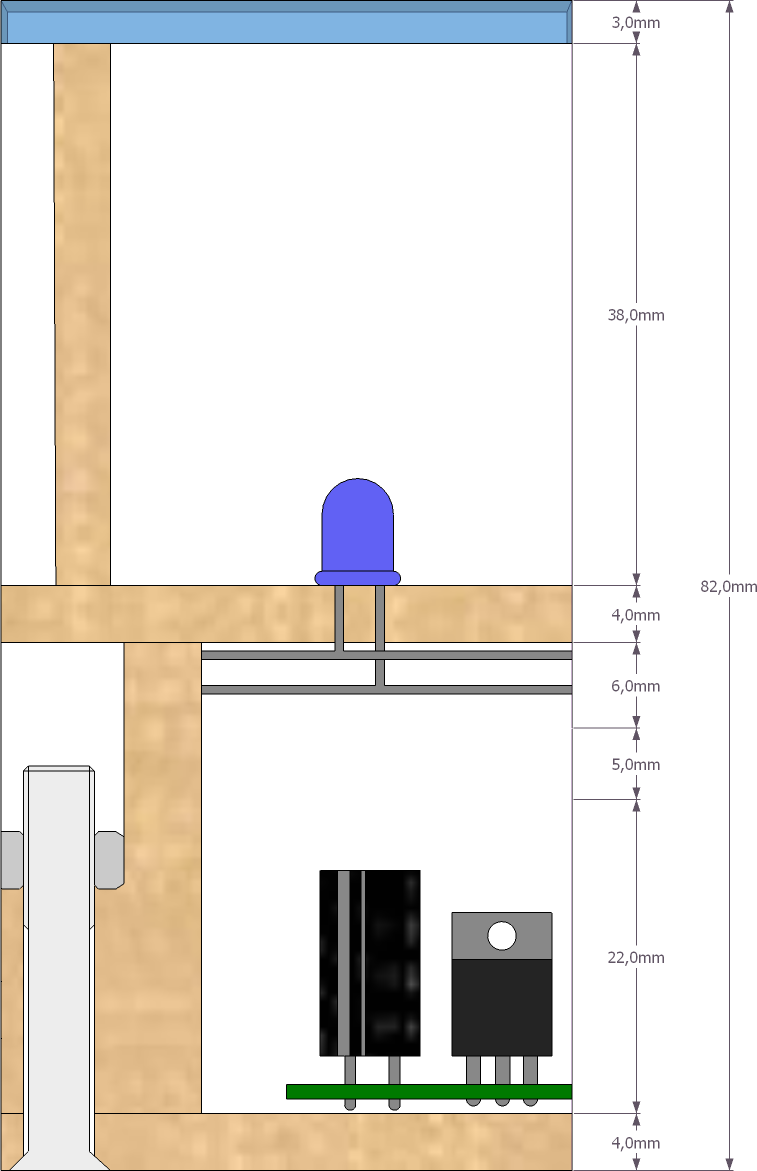
\includegraphics[width=0.6\textwidth]{skizzen/querschnitt.png}
\captionof{figure}{Schematischer Querschnitt des Gehäuses}
\label{fig_querschnitt}
\end{center}
Während der Entwicklung war ein einfacher Zugang von großer Bedeutung, deshalb wurde das Gehäuse in zwei Teile aufgeteilt. Die LED-Matrix bildet zusammen mit ihrer Abdeckung und drei Seitenwänden den vorderen Teil des Gehäuses. Auf der Rückwand wurde die Hauptplatine, das Netzteil und der DCF77-Empfänger platziert. An der vierten Seitenwand sind die Sensoren für Helligkeit und Temperatur, die Stromversorgung, die 6 Taster sowie der Debuganschluss (ISP) %TODO ISP als Fachwort
befestigt (siehe Abbildung \ref{fig_anschluesse}). Diese Seitenwand wurde an der Rückwand befestigt. Dies ermöglicht ein Öffnen des Gehäuses, indem nur die Schrauben an der Rückwand entfernt werden und die 3 Steckverbinder zur LED-Matrix gelöst werden, die komplette Sensorik und die Taster aber nicht entfernt werden müssen.%
\vspace{2em}
\centerline{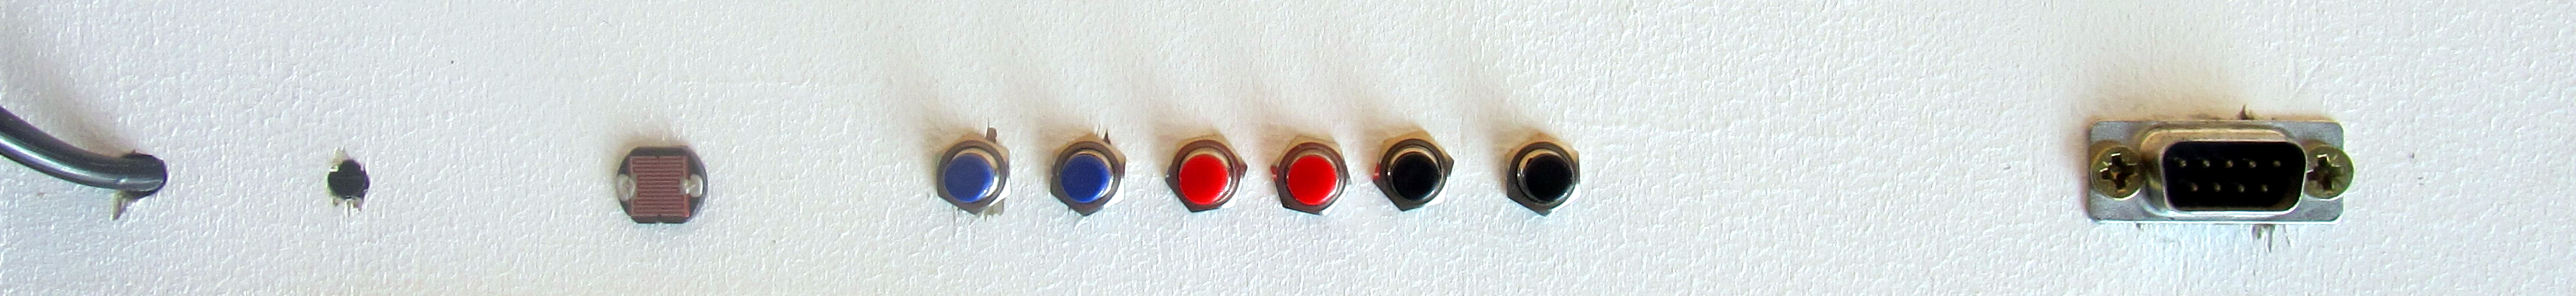
\includegraphics[width=\linewidth]{images/anschluesse.png}}
\captionof{figure}{Taster, Sensoren und ISP-Schnittstelle der Digitaluhr}\label{fig_anschluesse}
\vspace{.5em}
%TODO Fotos von dem ganzen Kram

Als Schrauben kamen Metallschrauben mit M5 %TODO 
Gewinde zum Einsatz. Die Muttern wurden in einem Holzblock befestigt, der anschließend mit der Rückwand verleimt wurde.%TODO: Abbildung? 
Diese Lösung zeichnet sich im Gegensatz zu Holzschrauben durch minimalen Verschleis aus und kann oft geöffnet und wieder verschlossen werden ohne Auszufransen.

\subsubsection{Energieversorgung und Verbrauch}
%TODO: Tabelle mit Alle AN/ Alle Aus/ Halb an. (eventuell mit neuen und alten Widerständen 
Als Netzteil wurde ein CE geprüftes 5V/2A Netzteil gewählt. Das kompakte verwendete Schaltnetzteil ist ausreichend dimensioniert um den, mit einem Labornetzteil, ermittelten maximalen Bedarf von ca. 1.8A%TODO
(alle LEDs an bei maximaler Helligkeit) bereitzustellen.
 
Als Stromkabel kommt ein zweipoliges Kabel mit Schalter zum Einsatz. Dieses wurde im Inneren des Gehäuses mit Schmelzklebestoff verklebt und in eine Lüsterklemme geführt, so dass bei eventuell auftretenden Zugkräften auf keinen Fall Kräfte auf das Netzteil wirken.

Mittels des Temperatursensors wurde außerdem in einem Testlauf sichergestellt, dass die Temperatur im Inneren der Uhr 50\degree C (bei einer Raumtemperatur von 22\degree C) nicht überschreitet.
%eof